% !TEX root = ProjetoPDS.tex
\section{Análise dos Sinais}

\subsection{Caracterização do Sinal}
\begin{figure}[H]
\centering
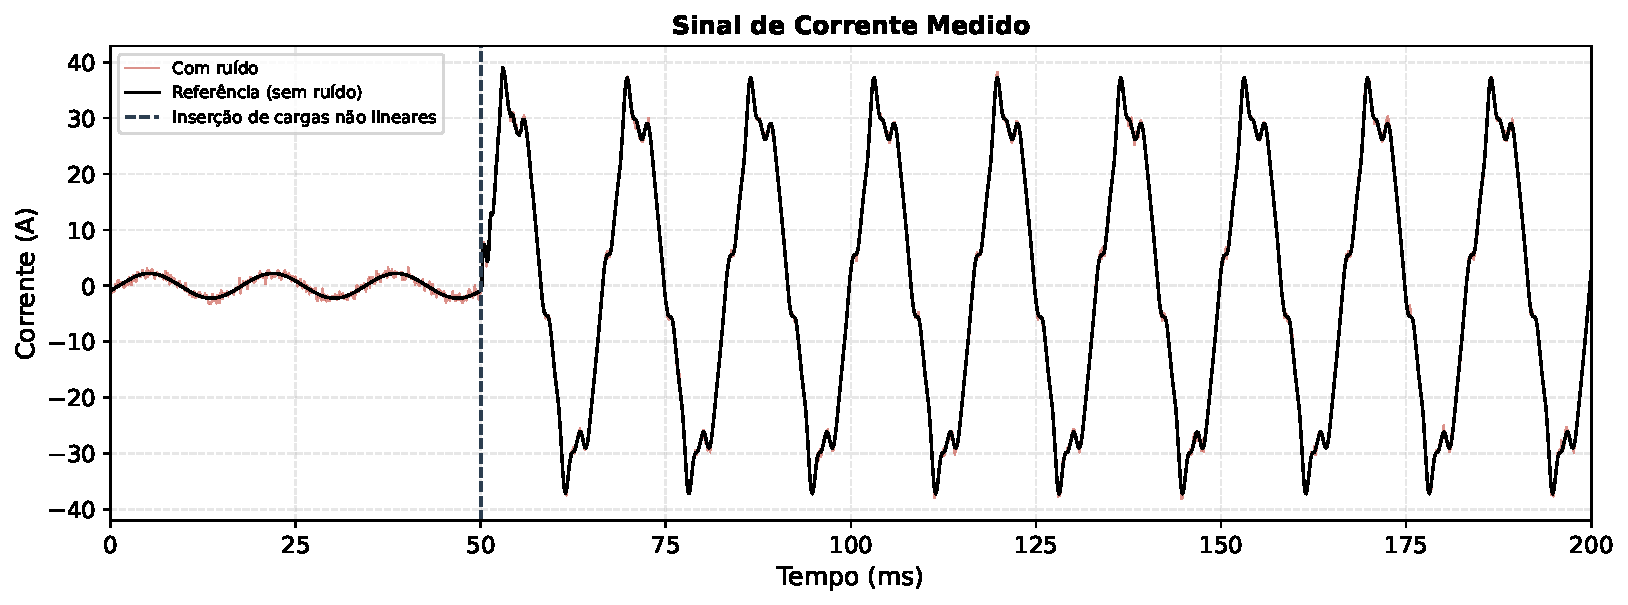
\includegraphics[width=\columnwidth]{sinal_bruto_b9.pdf}
\caption{Sinal de corrente medido (registro ruidoso e referência sem ruído), com
o instante de inserção das cargas não lineares destacado.}
\label{fig:sinal}
\end{figure}

O sinal possui \num{1537} amostras (\SI{0.20}{\second} a \SI{7680}{\hertz}) e
está reproduzido na Fig.~\ref{fig:sinal}, que mostra o registro ruidoso, a
referência sem ruído e o instante de inserção das cargas não lineares. Esse
instante foi localizado na amostra~384 ($t \approx \SI{50}{\milli\second}$) por um
detector de degrau da envoltória: calcula-se o valor eficaz (RMS) ciclo a ciclo da
fundamental (\num{128} amostras) e toma-se a maior variação entre ciclos
consecutivos. Nessa fronteira o RMS salta de \SI{1.57}{\ampere}, sob cargas
lineares, para \SI{23.1}{\ampere} após o chaveamento, confirmando a transição; a
filtragem proposta preserva esse transitório.

Distinguem-se dois regimes de operação. Antes do chaveamento, com cargas
lineares, a corrente é quase senoidal e de baixa amplitude (poucos ampères).
Depois da entrada das cargas não lineares, a amplitude cresce de repente
(fundamental de \SI{32.3}{\ampere}) e a forma de onda deixa de ser senoidal,
achatada pelos harmônicos de ordem $6k\pm1$. O desafio da filtragem é duplo: tirar
o ruído de medição, de banda larga, sem suavizar a distorção harmônica do segundo
regime, que é justamente a informação útil para a análise de qualidade de energia.

\subsection{Filtragem no Domínio do Tempo}
\begin{figure*}[t]
\centering

\includegraphics[width=0.92\textwidth]{resultado_filtros_iir_b9.pdf}
\caption{Filtragem no domínio do tempo: a melhor configuração de cada aproximação
sobre os sinais de referência e ruidoso (painéis superiores) e o erro residual
(filtrado menos referência) das quatro aproximações, sobreposto e ampliado no
transitório do chaveamento (painel inferior), fase zero.}
\label{fig:tempo}
\end{figure*}

A Fig.~\ref{fig:tempo} traz, nos quatro painéis superiores, o melhor filtro de cada
aproximação sobre os sinais de referência e ruidoso; na escala cheia as três curvas
ficam quase coincidentes --- efeito da filtragem eficaz e do ruído pequeno frente ao
sinal ---, evidenciando que o ruído é removido e a forma de onda preservada nos dois
regimes. O painel inferior amplia o \emph{erro residual} (filtrado menos referência)
das quatro aproximações na janela do chaveamento (amostras~300--460) --- a grandeza
minimizada pelo RMSE ---, justamente onde elas mais se distinguem: os filtros de
corte mais baixo (Chebyshev~I e elíptico, fc~$=700$~Hz) apresentam o maior
sobressinal e oscilação após o degrau --- passa-banda estreita implica resposta ao
impulso mais longa ---, enquanto o Chebyshev~II ($\star$, fc~$=2700$~Hz) reage de
forma mais contida, o que se reflete no seu menor RMSE. Fora desse transitório o erro
é pequeno (décimos de ampère) e semelhante nas quatro.

\subsection{Funções de Transferência e Estabilidade}
As duas melhores configurações de fase zero, ambas de ordem~3, possuem as funções
de transferência discretas
\begin{equation}
H_{\text{But}}(z) = \frac{0{,}0443 + 0{,}1328\,z^{-1} + 0{,}1328\,z^{-2} + 0{,}0443\,z^{-3}}
{1 - 1{,}2420\,z^{-1} + 0{,}7486\,z^{-2} - 0{,}1524\,z^{-3}},
\label{eq:hbut}
\end{equation}
\begin{equation}
H_{\text{Ch2}}(z) = \frac{0{,}0483 + 0{,}1141\,z^{-1} + 0{,}1141\,z^{-2} + 0{,}0483\,z^{-3}}
{1 - 1{,}3104\,z^{-1} + 0{,}8008\,z^{-2} - 0{,}1654\,z^{-3}}.
\label{eq:hch2}
\end{equation}

\begin{figure}[H]
\centering

\includegraphics[width=0.78\columnwidth]{polos_zeros_b9.pdf}
\caption{Diagrama de polos e zeros do filtro Chebyshev~II de ordem~3.}
\label{fig:polos}
\end{figure}

O filtro Butterworth tem polos em $0{,}447 \pm j0{,}487$ e $0{,}349$, com módulo
máximo $|p|_{\max} = 0{,}661$; o Chebyshev~II, em $0{,}475 \pm j0{,}482$ e
$0{,}361$, com $|p|_{\max} = 0{,}677$. Como todos os polos têm módulo inferior à
unidade, ambos são estáveis no sentido BIBO (entrada limitada, saída limitada). A
Fig.~\ref{fig:polos} exibe o diagrama do Chebyshev~II: os três polos ficam bem no
interior do círculo unitário, enquanto um par de zeros se posiciona sobre o
círculo ($-0{,}681 \pm j0{,}733$), criando os \emph{notches} de transmissão
característicos dessa aproximação; os três zeros do Butterworth, em contraste,
coincidem em $z = -1$. A Fig.~\ref{fig:resposta} apresenta a resposta em
frequência (magnitude) dos quatro filtros, e a Fig.~\ref{fig:espectro}, o efeito
da filtragem sobre o espectro do sinal.

\begin{figure*}[t]
\centering

\includegraphics[width=0.85\textwidth]{resposta_frequencia_b9.pdf}
\caption{Resposta em frequência (magnitude) dos melhores filtros.}
\label{fig:resposta}
\end{figure*}

\begin{figure*}[t]
\centering

\includegraphics[width=0.85\textwidth]{espectro_fft_b9.pdf}
\caption{Espectro de magnitude (FFT) antes e depois da filtragem.}
\label{fig:espectro}
\end{figure*}

\begin{figure}[H]
\centering

\includegraphics[width=\columnwidth]{custo_vs_ordem_b9.pdf}
\caption{RMSE e custo computacional em função da ordem do filtro.}
\label{fig:custo}
\end{figure}

Explique as parametrizações testadas para o algoritmo de processamento digital de sinais utilizado (se houver).

Demonstre, de preferência graficamente, as saídas do algoritmo de processamento digital de sinais utilizado. Ou traga valores tabelados. A Tabela~\ref{tab:results} exemplifica a tabulação de dados para apresentação de resultados.

\begin{table}[!h]
\renewcommand{\arraystretch}{1.2}
\caption{Dados tabulados.}
\label{tab:results}
\centering
\begin{tabular}{|c|ccccc|}
\hline
\multirow{2}{*}{\textbf{Zone}} & \multicolumn{5}{c|}{\textbf{MRE}} \\
 & \textbf{6-pulse} & \textbf{12-pulse} & \textbf{SFC} & \textbf{DC motor} & \textbf{TCR} \\
\hline
\textbf{1} & 15.2\% & 14.4\% & 32.2\% & 5.9\% & 35.2\% \\
\textbf{2} & 10.3\% & 12.0\%  & 7.1\% & 5.3\%  & 19.7\% \\
\textbf{3} & 0.6\% & 2.3\%  & 2.2\% & 1.3\%  & 0.5\% \\
\hline
\textbf{General} & 6.9\%  & 8.2\%  & 9.4\% & 3.7\%  & 14\% \\
\hline
\end{tabular}
\end{table}

Apresente e discuta os resultados finais de seu projeto. Pode usar gráficos e/ou tabelas. Entretanto, precisam ser devidamente explicados.
